\section{Discussion}
\label{sec:Discussion}
In the following discussion, the results presented in the previous section will be analysed more in-depth. Furthermore, qualitative results from the road detection system are evaluated, and might illustrate why methods for dealing with noisy labels are important for this type of dataset.\\

The \ac{CNN} and the proposed methods are in some sense comparable to the three groups of approaches for dealing with label noise, described in \ref{sec:background_label_noise}. The bootstrapping loss function is clearly a noise-tolerant approach, where the loss function is modified in an attempt to make the network more robust towards label noise. The \ac{CNN} and the regularization methods used, can be categorized as a noise-robust model. Whereas, curriculum learning in some sense can be described as a data cleansing method. The training set does not exclude any examples from all stages, or relabel examples. But, the ``simple" stages are created based on filtering techniques, where inconsistency between label and prediction determine whether an example is excluded from a training set stage.  \\

\subsection{The Effect of Bootstrapping}
Unfortunately, the effect of employing the bootstrapping loss function is quite small. However, the bootstrapping methods did perform nearly equal or slightly better when observing the breakeven values in Experiment E1, E2 and E3. And for increasing levels of omission noise,  as seen in Figure \ref{fig:E1_boot_mass}, and Figure \ref{fig:E2_boot_norway}, it seems that bootstrapping do exhibit some robustness towards label noise. Compared to the performance of the baseline, the difference in both test loss and breakeven seems to be increasing.  \\

Even though, up to 40\% of the roads present in the label images was removed, it did not particularly affect the baseline much. The baseline network seems to be surprisingly robust towards label noise. However, the default patch dataset sampling policy might be somewhat responsible for this.\\

In Experiment E1 and E2, only omission noise was artificially added to the label images. This simply removed road pixels from the label images, until a certain percentage of road pixels had been removed. However, when the patch creator sampled the aerial dataset for example patches, the preference for an even balance between patches containing road pixels and patches not containing any road pixels, was enabled. Even for increasing levels of omission noise, the patch creator still sampled around 50\% road patches with almost no noise added. The portion of non-road patches in the patch dataset was of course affected by the increase in label noise. Adding artificial but realistic registration noise to the label images were not done in the experiments. This would have affected the entire patch dataset. In appendix \todo{Add results in appendix}, the results from increasing levels of label noise by flipping label pixels are presented. In this scenario, bootstrapping is much more effective. Unfortunately this type of label noise is highly unrealistic for this type of dataset.\\

There is also the issue of seemingly contradictory results in Experiment E3. Even though bootstrapping in Figure \ref{fig:E3_boot_norway_vbase} shows an increase in the loss towards the end, it still achieves a better precision and recall curve than cross-entropy loss. This is probably an indication of bootstrapping actually working. It seems that the bootstrapping loss function slightly adjust the predictions to be more consistent between perceptually similar examples, at the cost of an increasing test loss. The Vbase test set labels are not perfect, and exhibit some registration and omission noise, which probably explains the increase in test loss. The bootstrapping function might be reducing the impact of local registration noise,  adjusting the predictions to fit the road pixels better. These prediction adjustments will be visible in the MSE loss, but will not affect the precision and recall because of the relaxed measure of precision. \\

The alternative bootstrapping loss function  behaves slightly different compared to bootstrapping, as demonstrated by the test loss figures, \ref{fig:E2_boot_norway_loss} and \ref{fig:E3_boot_norway_vbase_loss}. In these figures, the confident bootstrapping seems to follow the general outline of the baseline more closely than bootstrapping. The only difference between the two, is that the confident bootstrapping loss function modifies targets using only confident pixel predictions. In addition, for the N50 label set in Experiment E3, this loss function actually performed slightly better than bootstrapping and the baseline in terms of precision and recall. \\ 

In summary, the experiments show that the bootstrapping seem to something, but the performance difference between the loss functions is not statistically significant.\\

%An additional challenge was the constraint on runtime. To run 10 replicate experiments, the patch dataset size had to be limited. This might impact the performance of the bootstrapping methods, since they rely on models that have already incorporated some implicit knowledge about the data.\\

\subsection{Curriculum Learning by Using an Artificial Teacher}

All experiments comparing a randomly sampled patch dataset and a patch dataset constructed from a curriculum strategy, showed that presenting less difficulty examples first have a positive impact on the classifier's ability to generalize. Furthermore, the proposed curriculum strategy that are based on measuring disagreement between the labels and the predictions of a teacher classifier, seems to be a viable approach for conducting curriculum learning.\\

A benefit of using this particular curriculum strategy, is that it appears to be generally applicable. As long as a teacher classifier is trained to a certain level for a arbitrary dataset, it should be possible to create a curriculum dataset using the difficulty estimation, $d(y,q)$. However, it does require training an additional classifier, and the resulting quality of the curriculum dataset probably corresponds to the competency of the teacher classifier. For images this strategy is compelling, since judging the perceived difficulty of examples based on the actual image content is hard.\\

Experiment E4 and E5 demonstrated that the examples presented first do impact the final performance of the network. This is evident from both the precision and recall curve as well as the test loss. It is conceivable that the a less challenging training set distribution, puts the network in an advantageous area of parameter space. Even though the latter half of training for the curriculum tests were conducted on a training set with the same example distribution as the baseline tests, the starting advantage of curriculum learning was still preserved in the final performance.  \\

From Experiment E4, it is also clear that anti-curriculum learning does not provide the same advantage as curriculum learning. The performance in Figure \ref{fig:E4_curr_mass_loss} converges already at around epoch 25, with a test loss considerably higher than the baseline. It is only able to approach the test loss of the baseline after switching to the natural example distribution at epoch 50. The final test loss converged to a level well above the baseline. This also illustrates that the examples presented first, have a large influence on the outcome. It is possible that early optimization on harder examples, guides the network to an unfavourable local minima, which is hard to escape from later on.\\

The results further shows that the outcome of curriculum learning is sensitive to the threshold parameter $D_0$. Figure \ref{fig:E5_curr_norway_loss} reveals that decreasing threshold value $D_0$, diminishes the effect of curriculum learning. Decreasing the threshold value results in a smaller pool of eligible examples that can be included in a stage 0 training set, which in turn can reduce the training set variability.\\ 

A bit surprising are the results from Experiment E6, which showed that training with the first stage only, did better than curriculum learning. This indicates that the inexperienced teacher model, actually did a good job separating out the very hard and possibly inconsistent examples from the first stage. It also shows that the second stage probably contains a good amount of inconsistent examples which penalize the network incorrectly, and affect the outcome. Alternatively, this might indicate that the threshold parameter $D_0$ was set to a value which resulted in sufficient example variation in the first stage training set. The network is therefore able to generalize well to the task of road detection.\\

However, assuming that harder examples are inconsistent and exclude them entirely from the training set should be done with caution. This could lead to hard, but correctly labelled examples to be excluded, as well as unfamiliar examples that the curriculum teacher has not seen before. If the teacher classifier could accurately detect inconsistent labelling, there would be no reason for doing curriculum learning in the first place.\\ 

A potential reason for the large spike in test loss after a stage switch, is that the entire training set is suddenly replaced. As seen in the test loss of Figure \ref{fig:E6_gradual_loss}, gradually mixing in examples from smaller subsequent stages seems to alleviate this. The breakeven point for this test is also substantially higher than the baseline, the first-stage-only curriculum, and the inexperienced teacher classifier.\\

In summary, the composition of the first stage has a big effect on the outcome of training. The results demonstrate that the proposed curriculum strategy, which is based on estimating inconsistencies between labels and predictions, works well in practice.

\subsection{Performance of the Road Detection System}
The images in Figure \ref{fig:E7_performance} illustrate qualitatively the performance of the network with the best performance on the Massachusetts Roads Dataset. The prediction image in Figure \ref{fig:E7_model_predictions} has been stitched together from $16 \times 16$ prediction patches. For this particular test image, the model was able to identify the majority of the roads present, except for an almost imperceptible dirt road on the right side of the image. There are also some prediction errors, such as roads being disconnected, and prediction artefacts in the forest areas. However, the majority of the forest artefacts have low prediction probabilities, and can be removed by a threshold operation applied to the probabilities. For instance, the threshold value which results in the best precision and recall trade-off of the model was used to binarize the predictions in Figure \ref{fig:E7_hit_image}.\\

An interesting observation is that the model also correctly predicts small private roads leading up to houses, as seen in Figure \ref{fig:E7_performance}. Furthermore, the model detects construction roads in the upper left corner. Since these roads are not present in the label image, the model is penalized for making these predictions by the cross-entropy loss function.\\

The predictions errors are displayed in Figure \ref{fig:E7_hit_image}, where the road label pixels and road prediction pixels are superimposed on the aerial image. The road pixels that are coloured green, have been correctly predicted. Whereas, the red and blue coloured pixels show the prediction errors. The red pixels indicate areas in which the system failed to predict road, and the blue pixels show areas where the system incorrectly predicted road. Yet, the majority of the prediction errors are understandable, and arguably not actually errors at all. Most of the blue areas, covers pixels which depict asphalt surfaces, and some of the red areas have trees covering the road. However, a certain challenge is the amount of disconnected roads, which especially occur at road junctions and highway ramps. Possible reasons for this type of prediction errors can be the low frequency of junctions and ramps in the dataset or that the model capacity is inadequate. More results similar to Figure \ref{fig:E7_performance}, can be found in Appendix \ref{app:roaddetectionresults}.\\



\begin{figure}
\begin{subfigure}{0.48\textwidth}
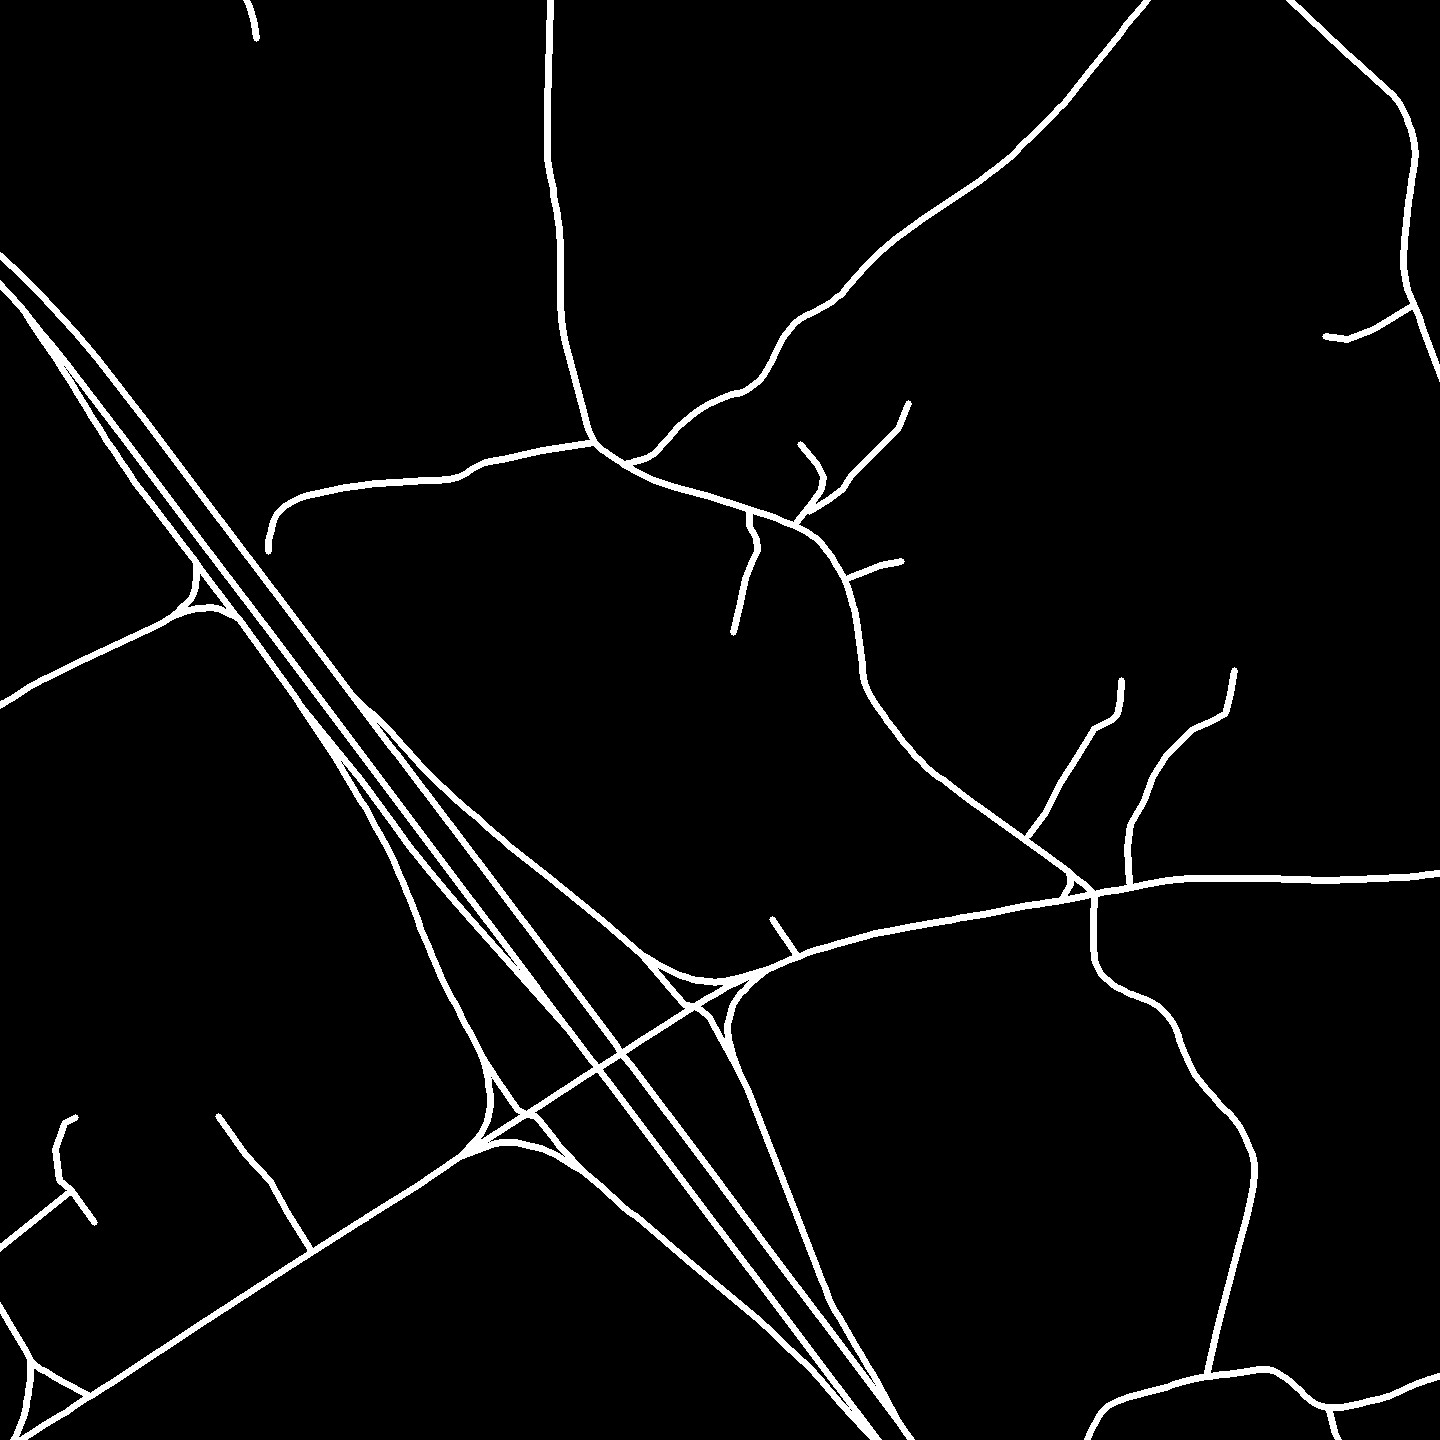
\includegraphics[width=\textwidth]{figs/E7/E7-label.jpg}
\caption{Label image.} \label{fig:E7_label_iamge}
\vspace{0.5cm} % separation vertically between the subfigures
\end{subfigure}
\hspace*{\fill} % separation between the subfigures
\begin{subfigure}{0.48\textwidth}
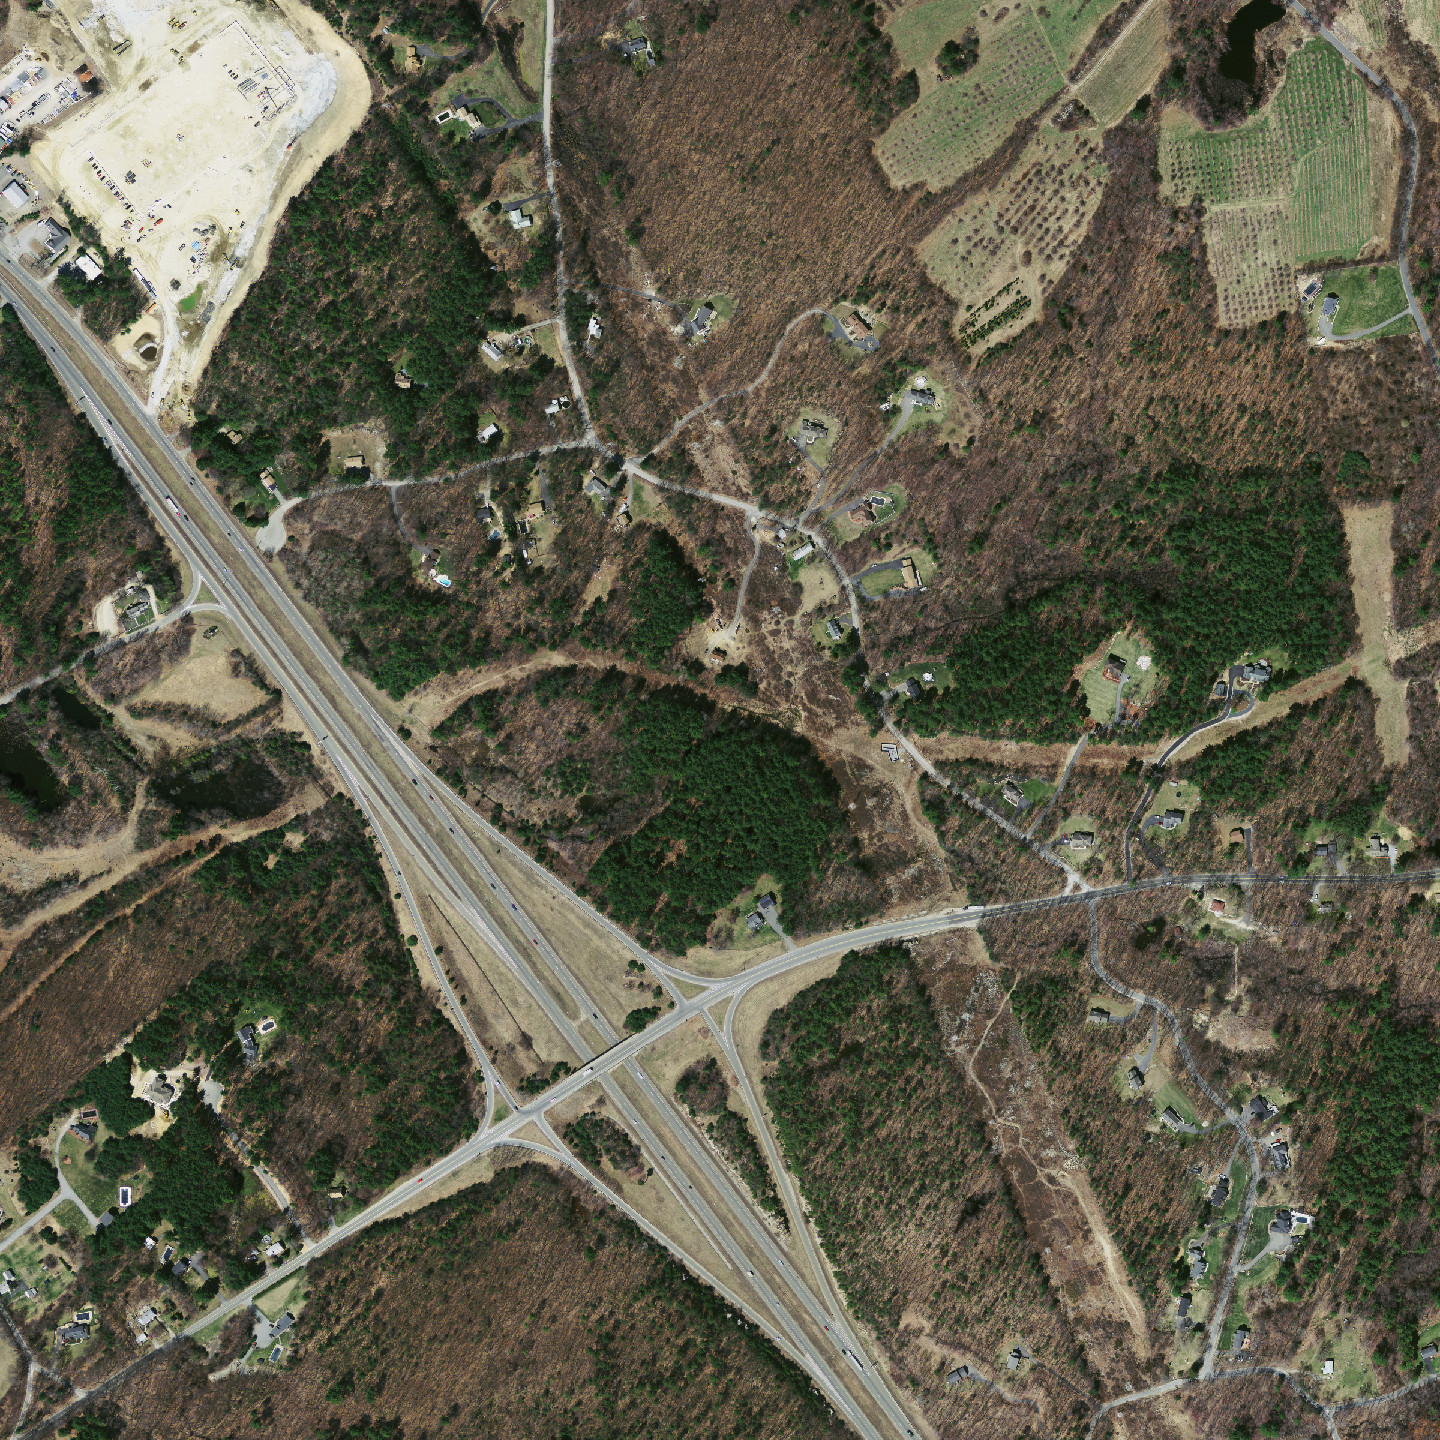
\includegraphics[width=\textwidth]{figs/E7/E7-image.jpg}
\caption{Aerial image.} \label{fig:E7_aerial_image}
\vspace{0.5cm} % separation vertically between the subfigures
\end{subfigure}

\begin{subfigure}{0.48\textwidth}
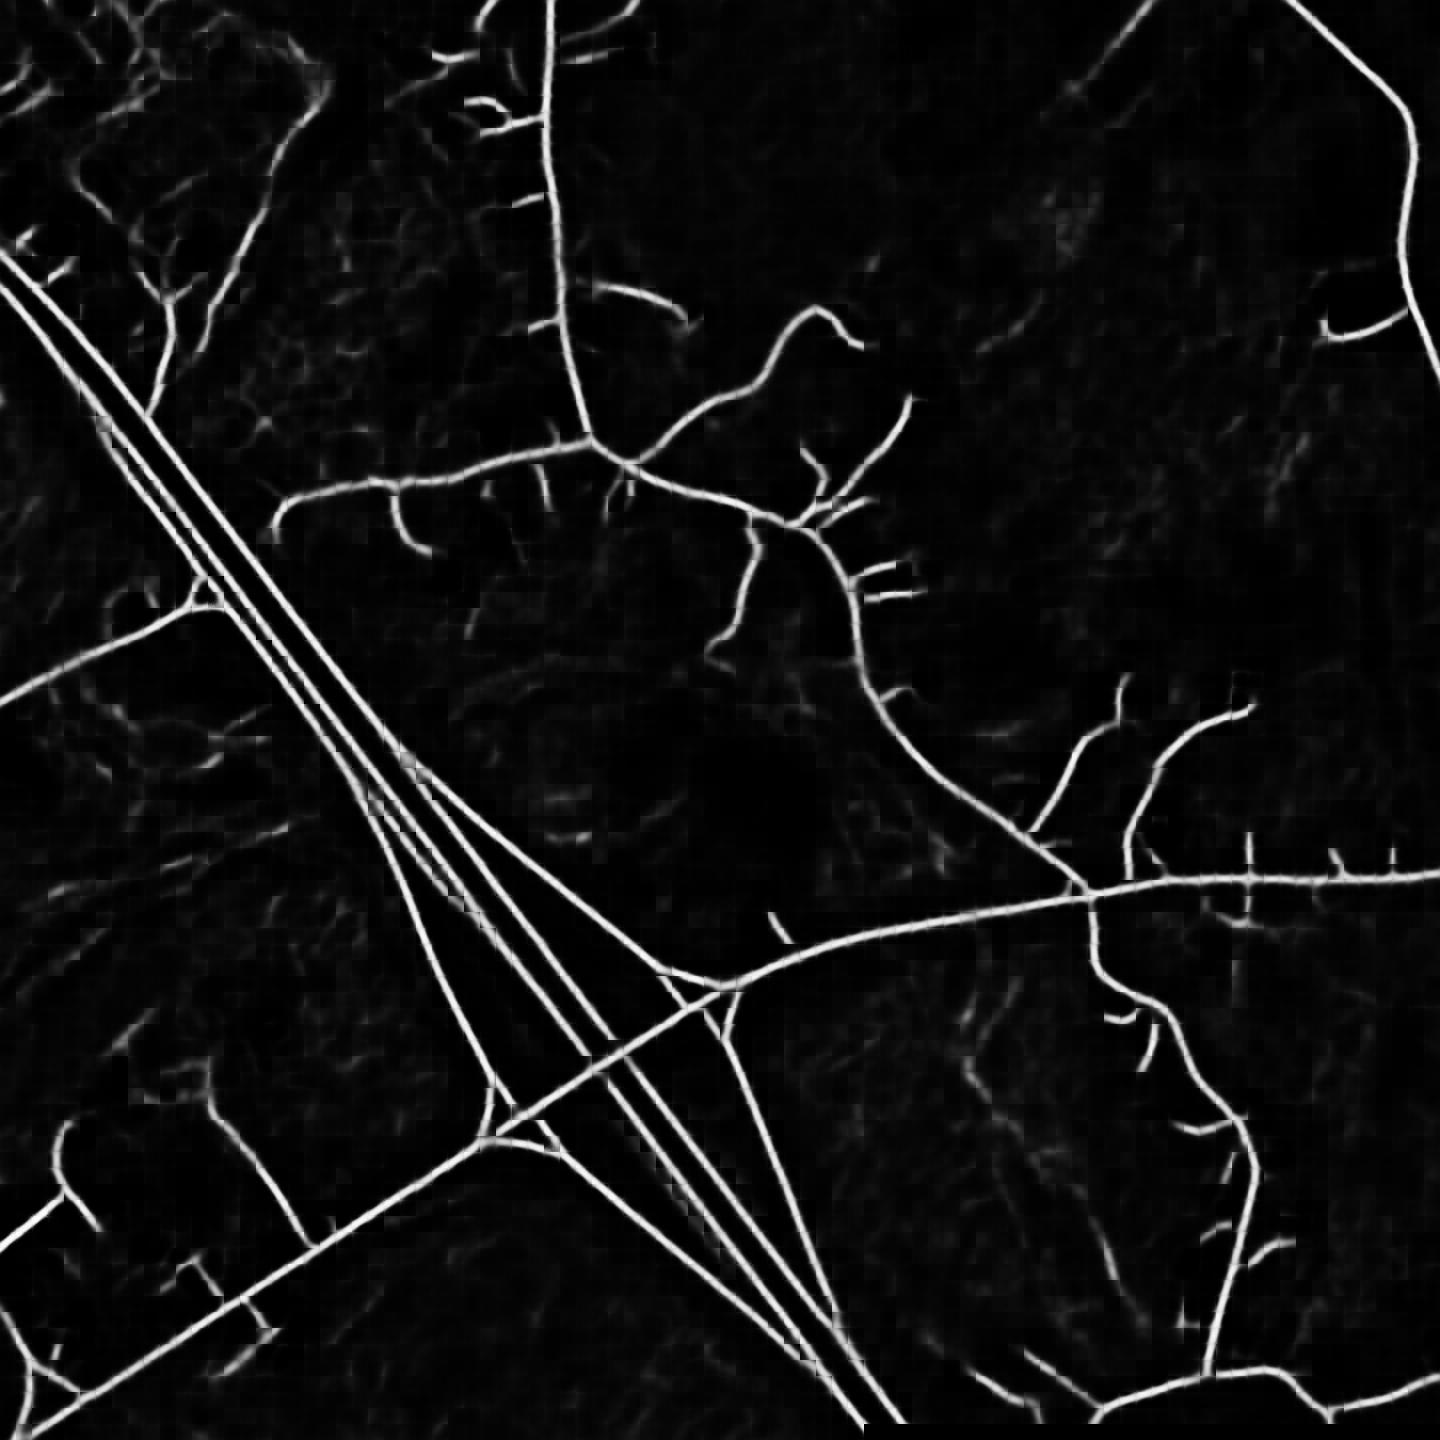
\includegraphics[width=\textwidth]{figs/E7/E7-pred.jpg}
\caption{Model predictions.} \label{fig:E7_model_predictions}
\end{subfigure}
\hspace*{\fill} % separation between the subfigures
\begin{subfigure}{0.48\textwidth}
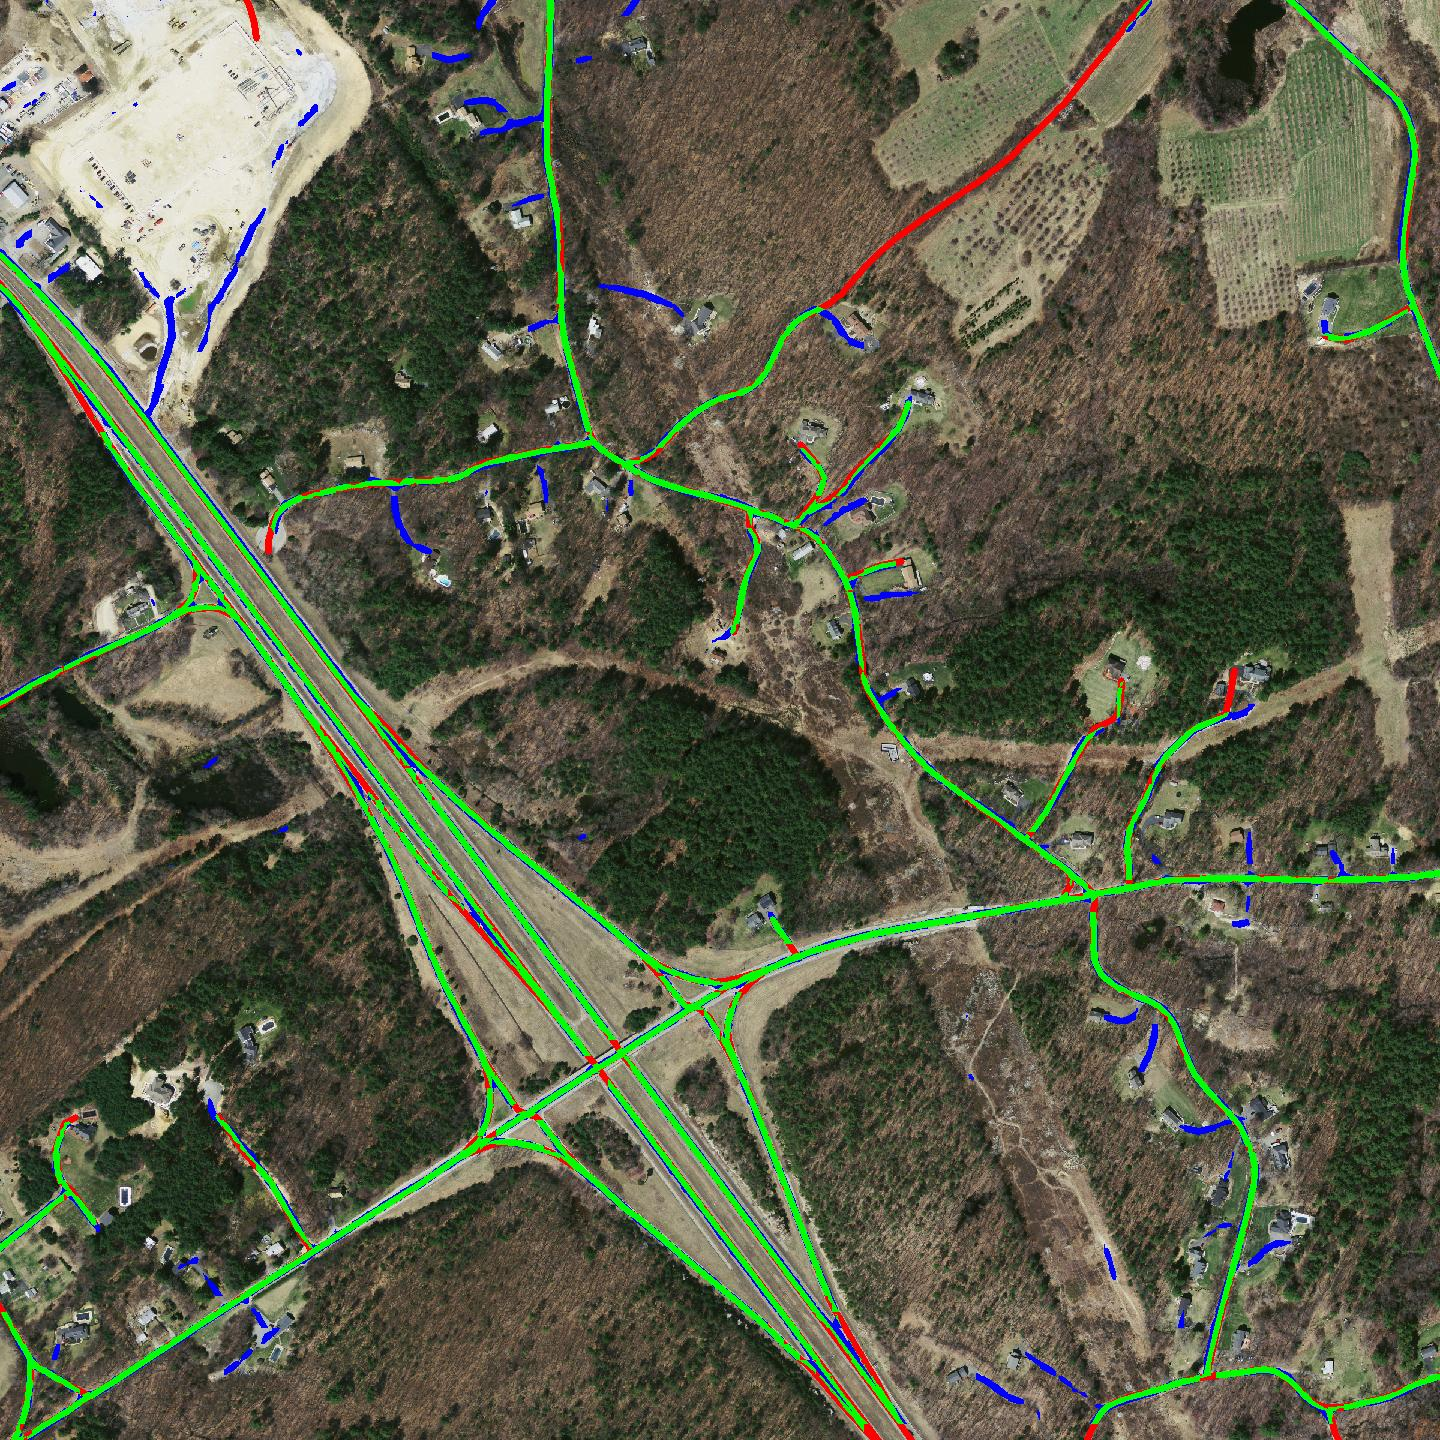
\includegraphics[width=\textwidth]{figs/E7/E7-hit.jpg}
\caption{Prediction hit and miss image.} \label{fig:E7_hit_image}
\end{subfigure}
\caption[E7 - Qualitiative results of the road extraction system ]{E7 - Example of model's road detection performance. The aerial image is part of the test set in Massachusetts Roads Dataset} \label{fig:E7_performance}
\end{figure}

One of the most compelling ways of reducing the disconnected roads errors, is utilizing structured output prediction methods, as discussed in \ref{sec:related_works}. Several studies \citep{Kluckner_semantic_height} \citep{LeCun_semantic} \citep{Mnih_roads_high_res_aerial_images} have shown that employing a smoothness prior by taking neighbouring predictions into account, can significantly improve generalization in semantic segmentation tasks. This is unfortunately outside the scope of this thesis.\\

The precision and recall breakeven point of M1 is considerably lower compared to other works, as seen in Table \ref{tab:results_curriculum_learning_breakeven}. The most likely explanation is the network configuration of this network. The configuration of the first layer in the network trained by \citep{MnihThesis} was different. \citep{MnihThesis} used overlapping max pooling in the first layer, whereas the max pooling of M1 was non-overlapping. This resulted in fewer learnable parameters in M1, which could have affected the network's model capacity, or ability to fit the data. The spatial reduction of the input in the first convolutional layer especially affects the number of incoming connections to the first fully connected layer of the network.  The network by \cite{MnihThesis} has approximately 17.3 million adjustable weights.\\

This was tested in Network M2, which used a different stride and kernel sizing. The number of adjustable weights in this network was around 5 million compared to around 1.6 million in Network M1. A large portion of the difference can be traced back to the large increase in incoming connections to the fourth layer. The incoming connections in M1 was 80, compared to 720 in M2. This network achieved a precision and recall breakeven point of 0.8494, even though it was trained with fewer examples and for less epochs. In addition, this network was trained using a gradual curriculum strategy, and used the confident bootstrapping loss function. \\

The same network configuration, loss function and training regime was tested with the Norwegian Roads Dataset Vbase in Network N1. The precision and recall breakeven point of this network was substantially lower. There are probably several reasons for this. First, the lower \ac{GSD} of this dataset implies that patches of $64 \times 64$ pixels convey less context compared to similarly sized patches from the Massachusetts Roads Dataset. This might reduce the network's ability to discriminate between road and non-road pixels in situations where surrounding context is key. Second, the results from the two roads datasets can not be directly compared, because they are different. The Norwegian Roads Dataset has images of varying image quality, and depict a wide range of topographical features. Furthermore, The Vbase label set has been rasterized with ill-suited line thichnesses for roads that are particularly wide or narrow. The examples in Figure \ref{fig:ill-suited} illustrate this. 

\begin{figure}
\begin{subfigure}{0.28\textwidth}
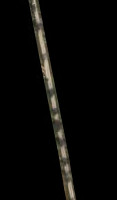
\includegraphics[width=0.73\textwidth]{figs/illsuited_label.jpg}
\caption{Non-road pixels superimposed.} \label{fig:ill-suited_example1}
\vspace{0.5cm} % separation vertically between the subfigures
\end{subfigure}
\hspace*{\fill} % separation between the subfigures
\begin{subfigure}{0.58\textwidth}
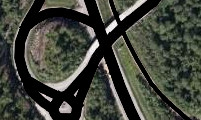
\includegraphics[width=\textwidth]{figs/illsuited_label2.jpg}
\caption{Road pixels superimposed.} \label{fig:ill-suited_example2}
\vspace{0.9cm} % separation vertically between the subfigures
\end{subfigure}

\caption[Examples of ill-suited line thickness]{Examples of ill-suited line thickness.} \label{fig:ill-suited}
\end{figure}
